% ****** Start of file aipsamp.tex ******
%
%   This file is part of the AIP files in the AIP distribution for REVTeX 4.
%   Version 4.1 of REVTeX, October 2009
%
%   Copyright (c) 2009 American Institute of Physics.
%
%   See the AIP README file for restrictions and more information.
%
% TeX'ing this file requires that you have AMS-LaTeX 2.0 installed
% as well as the rest of the prerequisites for REVTeX 4.1
% 
% It also requires running BibTeX. The commands are as follows:
%
%  1)  latex  aipsamp
%  2)  bibtex aipsamp
%  3)  latex  aipsamp
%  4)  latex  aipsamp
%
% Use this file as a source of example code for your aip document.
% Use the file aiptemplate.tex as a template for your document.
\documentclass[%
 aip,
% jmp,
% bmf,
% sd,
% rsi,
 amsmath,amssymb,
%preprint,%
 reprint,%
%author-year,%
%author-numerical,%
% Conference Proceedings
]{revtex4-1}

\usepackage{graphicx}% Include figure files
\usepackage{dcolumn}% Align table columns on decimal point
\usepackage{bm}% bold math
%\usepackage[mathlines]{lineno}% Enable numbering of text and display math
%\linenumbers\relax % Commence numbering lines

\usepackage[utf8]{inputenc}
\usepackage[T1]{fontenc}
\usepackage{mathptmx}
\usepackage{etoolbox}
\usepackage{mathtools}
\usepackage{amsfonts}
%% Apr 2021: AIP requests that the corresponding 
%% email to be moved after the affiliations
\makeatletter
\def\@email#1#2{%
 \endgroup
 \patchcmd{\titleblock@produce}
  {\frontmatter@RRAPformat}
  {\frontmatter@RRAPformat{\produce@RRAP{*#1\href{mailto:#2}{#2}}}\frontmatter@RRAPformat}
  {}{}
}%
\makeatother
\newcommand{\cchevrons}[1]{\langle\!\langle #1 \rangle\!\rangle}
\DeclarePairedDelimiter\abs{\lvert}{\rvert}
\DeclarePairedDelimiter\norm{\lVert}{\rVert}
\begin{document}

\preprint{AIP/123-QED}

\title[]{A Kinetic interpretation of the Frank's constant in calamitic fluids}
% Force line breaks with \\
\author{U. Zerbinati}
 %\altaffiliation[Also at ]{Physics Department, XYZ University.}%Lines break automatically or can be forced with \\
%\author{B. Author}%
 %\email{Second.Author@institution.edu.}
%\affiliation{ 
%Authors' institution and/or address%\\This line break forced with \textbackslash\textbackslash
%}%

%\author{C. Author}
 %\homepage{http://www.Second.institution.edu/~Charlie.Author.}
%\affiliation{%
%Second institution and/or address%\\This line break forced% with \\
%}%
\date{\today}% It is always \today, today,
             %  but any date may be explicitly specified

\begin{abstract}
\end{abstract}

\maketitle

\section{\label{sec:intro}Introduction}
In Ref.~\onlinecite{FRZ23} a kinetic approach to obtain hydrodynamic equations for calamitic fluids has been investigated, with the aim to derive an inviscid and compressible variant of the well-kown Leslie-Eriksen equations.
In the process, a kinetically motivated variant energy for the orientational degrees of freedom was proposed, in the absence of extern-field i.e.
\begin{equation}
\label{eq:OseenFrankGen}
\mathcal{I}[\vec{n}]\coloneqq \int_{\Omega} \cchevrons{\vec{\omega} \cdot \mathbb{I}\vec{\omega}}\,d\vec{x},
\end{equation}
where $\mathbb{I}$ is the microscopic inertia tensor and the symbol $\cchevrons{\cdot}$ denotes the average over the microscopic: linear momentum $\vec{p}$, euler angles $\vec{\alpha}$ and their conjugate moments $\vec{\varsigma}$, weighted by the a priori unknown one-particle distribution $f(\vec{q},\vec{p},\vec{\alpha},\vec{\varsigma},t)$, i.e.~
\begin{equation}
	\cchevrons{\cdot} \coloneqq \frac{1}{n}\int\!\!\!\int\!\!\!\int\psi\,f({\vec{q}},\vec{p},\vec{\alpha},\vec{\varsigma},t)\,d\vec{v}d\vec{\alpha}d\vec{\varsigma}.
\end{equation}
Notice that phase-space, which variable we here denote $\Gamma=(\vec{\xi},\vec{\pi})=(\vec{q},\vec{p},\vec{\alpha},\vec{\varsigma})$, over which the one-particle distribution is evaluated is larger compared to the one for the classical Boltzmann equation, this because rotational degree of freedom $\vec{\alpha}$ and their conjugate moments $\vec{\varsigma}$ had to be considered in order to describe the configuration of a calamitic molecule.

Near the thermodynamical equilibrium we can evaluate $\cchevrons{\vec{\omega}\cdot \mathbb{I}\vec{\omega}}$ using the Maxwell-Boltzmann distribution, i.e. the one-particel $f^{(0)}(\vec{\alpha},\vec{v},\vec{\varsigma})$ distribution such that the collision operator vanish.
The Maxwell-Boltzmann distribution for calamitic molecules can be dervied from microscopical consideration to be,
\begin{equation}
  \label{eq:MaxwellBoltzmann}
  f^{(0)}(\vec{\alpha},\vec{V},\vec{\Omega})=\frac{m^{\frac{3}{2}}(I_1I_2I_3)^{\frac{1}{2}}}{(2\pi k_B T)^3}\exp\Big[-m\frac{\abs{\vec{V}}^2}{2 k_B T}-\frac{\vec{\Omega}\cdot\mathbb{I}\vec{\Omega}}{2k_B T}\Big]
\end{equation}
normalised multiplyinng by $\frac{nQ\sin(\alpha_2)}{\int_{\mathbb{R}^3}Q\sin(\alpha_2)\,d\alpha}$ where $Q$ is defned as 
\begin{equation}
  Q=\exp\left(\frac{\vec{\omega}_0\cdot \mathbb{I}\vec{\omega}_0}{\frac{2}{3}\cchevrons{\theta}}\right)
\end{equation}
and both $\omega_0$ and the kinetic temperature $T$ are assumed to remain constant at equilibrium\cite{C56,CD63}.

A well-known result in kinetic theory is that the Maxwell-Boltzmann distribution can be rewritten in terms of the microscopic collision invariants alone\cite{FM}, hence the only order parameters appearing in the energy $\mathcal{I}$ must come from the $\mathbb{I}$.
To see this let us consider first the excluded volume interaction potential $\vec{U}(\vec{q}_1,\vec{q}_2,\vec{\alpha}_1,\vec{\alpha}_2)$, which is well-known to conserve:
\begin{enumerate}
  \item the total linear momentum, i.e. $p$,
  \item the angular momentum, i.e. $\frac{1}{m}(\vec{q}\times \vec{p})+\mathbb{I}\vec{\omega}(\vec{\alpha},\vec{\varsigma})$,
  \item the total kinetic energy, i.e. $\frac{1}{2m}\vec{p}\cdot \vec{p}+\frac{1}{2}\vec{\omega}(\vec{\alpha},\vec{\varsigma})\cdot \mathbb{I}\vec{\omega}(\vec{\alpha},\vec{\varsigma})$.
\end{enumerate}
When considering an excluded volume interaction, thanks to the nature of the microscopic collision invariants it is trivial to see that the order parameter only plays a role in $\mathbb{I}$.
Interestingly enough the above-defined collision invariants are also the invariants for any two-body interaction occurring as a result of a radial and orientationally invariant intermolecular potential, as for example the Gay-Berne potential\cite{GB81}.
In fact the Lagrangian of this two-body interaction
\begin{align}
  \mathcal{L}(\vec{\Gamma}_1,\vec{\Gamma}_2)=\frac{1}{2m}(p_1^2+p_2^2)&+\frac{1}{2}\vec{\omega}_1(\vec{\alpha}_1,\vec{\varsigma}_1)\cdot \mathbb{I}\vec{\omega}_1(\vec{\alpha}_1,\vec{\varsigma}_1)\nonumber\\
  &+\frac{1}{2}\vec{\omega}_2(\vec{\alpha_2},\vec{\varsigma}_2)\cdot \mathbb{I}\vec{\omega}_2(\vec{\alpha}_2,\vec{\varsigma}_2)\nonumber\\,
  &+U(\abs{\vec{q}_1-\vec{q}_2},\alpha),
\end{align}
is invariant under the translation and rotation hence applying Noether's theorem
\begin{equation}
  \label{eq:Noether}
  \frac{d}{dt}\left(\frac{\partial \mathcal{L}}{\partial \dot{\vec{\xi}}_{1,2}}\cdot G_i\right)=0, \qquad i=1,2,
\end{equation}
where $G_i$ are the generators of the translation and rotation group, i.e. $G_1=(1,1,0,0)$ and for an arbitrary unit-vector $\vec{n}$, $G_2=(\vec{n}\times \vec{q},\vec{n}\times\vec{q},1,1)$. In particular, we remark that \eqref{eq:Noether} with $G_1$ gives the conservation of the total linear momentum, while with $G_2$ the conservation of the total angular momentum.
Lastly, the conservation of the total kinetic energy is a direct consequence of the fact that the Lagrangian is time-independent and its kinetic energy portion is a homogeneous positive definite quadratic form of the generalized velocities\cite{FM}.
information
While at first, it might not appear obvious there are interesting consequences of the above observation. Not only the order parameters can come into play only through the inertia tensor, but for this reason the microscopic mechanism resulting in macroscopic anisotropic behavior in a calamitic fluid near the thermodynamical equilibrium is only determined by the geometrical about the calamitic constituents encoded in the inertia tensor.
\section{Needle-like molecules}
In Ref.~\onlinecite{FRZ23} a particular case of the energy \eqref{eq:OseenFrankGen} was considered in greater detail, i.e. the case of needle-like cilindircal molecules for which the inertia tensor can be written as
\begin{equation}
  \label{eq:InertiaTensor}
  \mathbb{I} \approx \lambda(I-\vec{n}\times \vec{n}),
\end{equation}
where $K\approx \mathcal{O}(\gamma h^2)$ for a needle-like molecule of length $h$ and $\vec{n}$ is the usual nematic director field. Under the assumption that the molecule is cylindrical we can use $\gamma\approx \frac{1}{12}$.
Under this hypothesis and using the Maxwell-Boltzmann distribution \eqref{eq:MaxwellBoltzmann} to evaluate the energy \eqref{eq:OseenFrankGen} near the thermodynamical equilibrium, it was shown\cite{FRZ23} that $\mathcal{I}$ can be written as
\begin{equation}
  \label{eq:OseenFrankOne}
  \mathcal{I}[\vec{n}]=\int_\Omega p\frac{\lambda}{2}\,\nabla\vec{n}:\nabla\vec{n}\,d\vec{x},
\end{equation}
where we have dropped all the non-spatially dependent terms and $p$ is the thermodynamical pressure exerted by the calamitic constituents of the fluid. Notice that under isobaric conditions \eqref{eq:OseenFrankOne} is the one-constant variant approximation of the well-known Oseen-Frank energy\cite{V}.
We would like to point out that \eqref{eq:OseenFrankOne} gives a very rudimental equation to compute the one-constant approximation $K$ of the Frank's constants, i.e.
\begin{equation}
  \label{eq:FrankConstant}
  K=\lambda p.
\end{equation}
Let us look at a few examples to see if \eqref{eq:FrankConstant} provides a good ``ball-park'' park estimate for $K$.

We begin by considering para-Azoxyanisole (PAA), which is a calamitic molecule known to form a nematic phase at sufficiently high temperatures.
From a steric point of view, PAA can be considered as a needle-like molecule with a length $h\approx 20 \overset{\circ}{A}$ and a diameter $d\approx 5 \overset{\circ}A$\cite{dGJ}.
Furthermore, PAA is a solid compound that when heated up forms a nematic liquid crystal phase around $120\,C^\circ$ and $1.6\cdot 10^{7} \text{Pa}$\cite{dGJ,DCJ71}.
Using \eqref{eq:FrankConstant} we can provide a rough estimate for $K$, i.e.
\begin{equation}
  K_{PAA} \approx 33.3 \cdot 1.6\cdot 10^{-13} \text{N} \approx 5.3\cdot 10^{-7} \,\text{dyn}.
\end{equation}
This value is in good agreement with the experimental value for which $K_1\approx 0.7\cdot 10^{-6}\,\text{dyn}$, $K_2\approx 0.43\cdot 10^{-6}\,\text{dyn}$ and $K_3\approx 1.7 \cdot 10^{-6}\,\text{dyn}$\cite{dGJ}.

We now consider N-(4-methoxybenzylidene)-4-butylaniline (MBBA), which is another calamitic molecule known to form a nematic phase at room temperature. MBBA can be considered as a needle-like molecule with a length $h\approx 70 \overset{\circ}{A}$ if regarded as a rigid cylindrical body\cite{CRB71}.
At atmospheric pressure, MBBA forms a nematic phase from $20\,C^\circ$ to $47\,C^\circ$, therefore using \eqref{eq:FrankConstant} we can provide a rough estimate for $K$, i.e.
\begin{equation}
  K_{MBBA} \approx 408.3 \cdot 1.01\cdot 10^{-15} \,\text{N}\approx 4.12\cdot 10^{-8} \, \text{dyn}. 
\end{equation}

Lastly, we consider 4-pentyl-4'-cyanobiphenyl (5CB), which can be regarded as a needle-like molecule with height $h\approx 20 \overset{\circ}{A}$\cite{Z} which forms a nematic phase from $22.5\,C^\circ$ to $35\,C^\circ$ at atmospheric pressure.
Hence once again using \eqref{eq:FrankConstant} we can provide a rough estimate for $K$, i.e.
\begin{equation}
  K_{5CB} \approx 33.3 \cdot 1.01\cdot 10^{-15} \,\text{N}\approx 3.3\cdot 10^{-8} \, \text{dyn}.
\end{equation}

\begin{figure}
  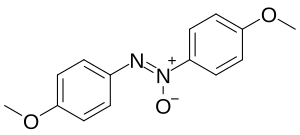
\includegraphics[scale=0.4]{Figures/PAA}\\
  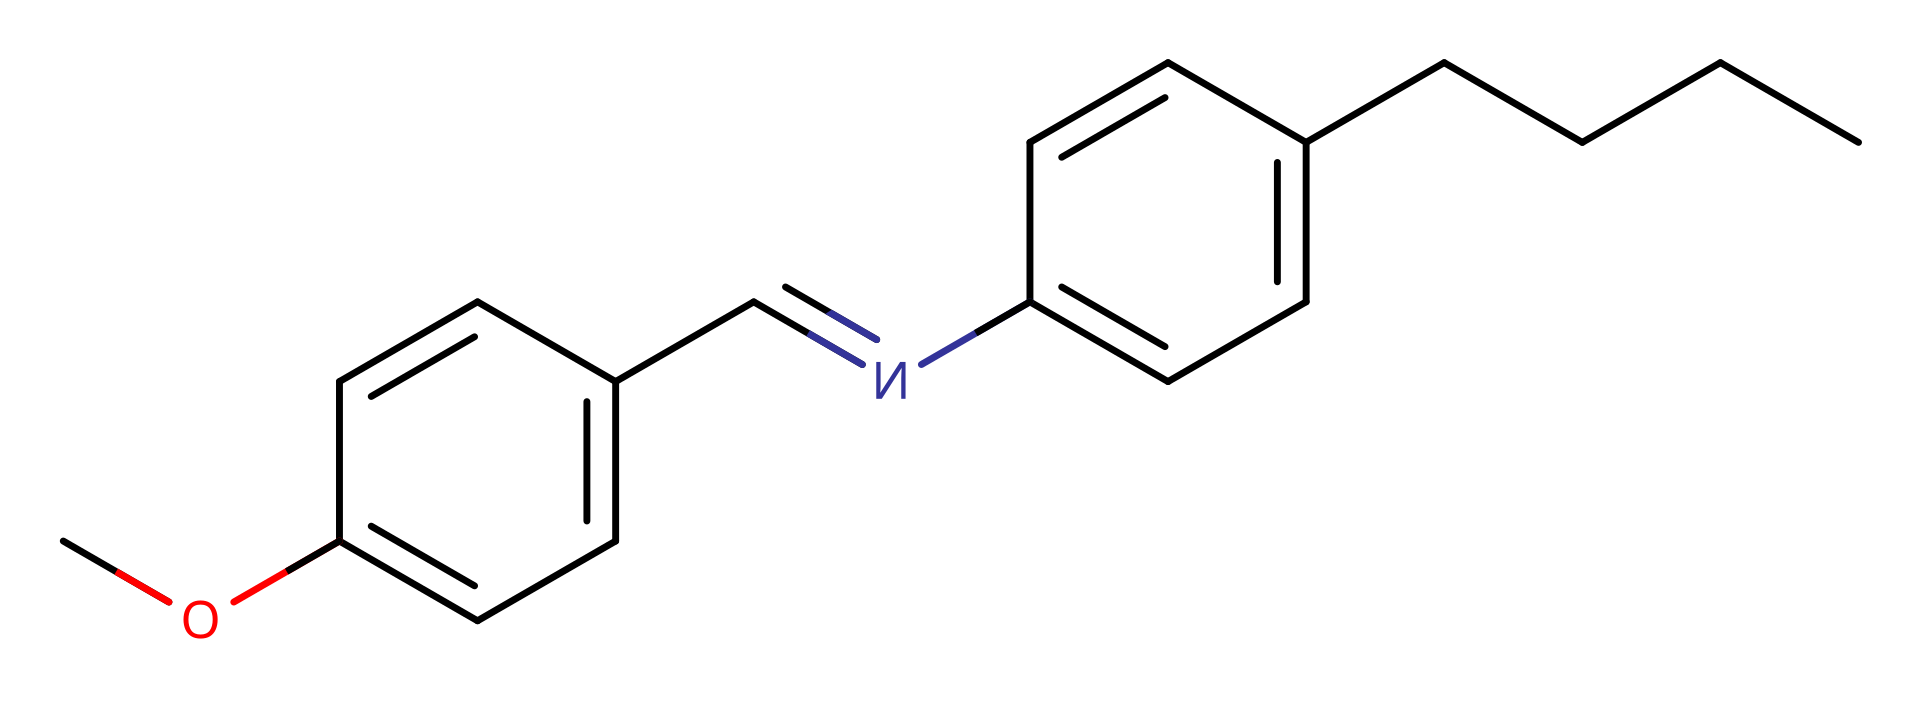
\includegraphics[scale=0.11]{Figures/MBBA}
  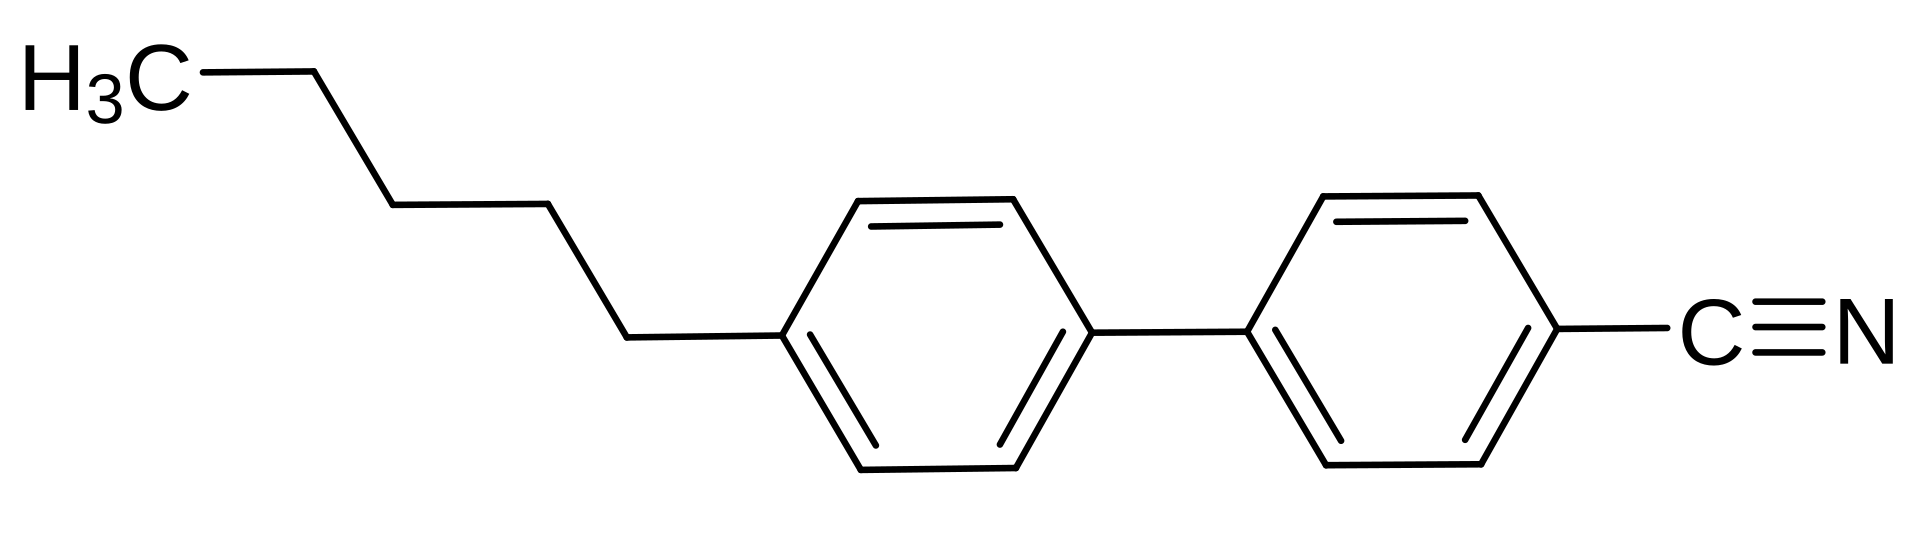
\includegraphics[scale=0.085]{Figures/5CB}
  \caption{In this figure are depicted the chemical structure of PAA, MBBA and 5CB liquid crystal.}
\end{figure}

While for PAA, \eqref{eq:FrankConstant} provided a good one constant approximation of Frank's constants, the same can not be concluded for MBBA and 5CB for which \eqref{eq:FrankConstant} understimates the Frank constant by one order of magnitude.
Looking at Figure \ref{fig:chem} a possible explanation come to mind, i.e. while the chemical structure of PAA seems to be almost head-to-tail symmetric and therefore we can regard it as a needle-like cylinder the same can not be said for MBBA and 5CB.
One idea can be to regard MBBA and 5CB as needle-like cones, where the adjective needle-like refers to the fact that we assume \eqref{eq:InertiaTensor} still holds, yet since we are assuming the molecule has a cone shape $\gamma\approx\frac{3}{5}$.
Using this assumption we obtain,
\begin{equation}
  K_{MBBA} \approx 3.7 \cdot 10^{-7}\,\text{dyn}, \qquad K_{5CB}\approx 2.9\cdot 10^{-7}\,\text{dyn}.
\end{equation}
These values are more inline with the experimental measure of Frank's constants for MBBA, for which $K_1 \approx 5.3 \cdot 10^{-7}\,\text{dyn}$, $K_2 \approx 2.2 \cdot 10^{-7}\,\text{dyn}$, $7.5\cdot 10^{-7}\, \text{dyn}$\cite{dGJ}, and 5CB for which $K_1\approx 3.5\cdot 10^{-7}\,\text{dyn}$ and $K_3\approx 4.15\cdot 10^{-7}\,\text{dyn}$\cite{BRBF85}.
\section{Pressure and Temperature dependence}
An interesting consequence of \eqref{eq:FrankConstant} is that the it predicts that Frank constant will increase lienarly with the pressure. A positive correlation between Frank's constants and pressure has been observed also experimentally\cite{SBF87}, in particular the experimental data presented in Ref. \cite{PRPH12} we can confirm the linear dependence describe by \eqref{eq:FrankConstant}, for the beding and splay constants.

On the other hand it is a well-known fact that the magnitude of the Frank constants decrease as the temperature increases\cite{dGJ,G73}.
\bibliography{aipsamp}
\end{document}